\documentclass[./Thesis]{subfiles}


\graphicspath{{./Images/}}
\begin{document}
\chapter{E989 Experiment at Fermilab}

In this chapter there will be an explanation of the experimental apparatus used for the E989 experiment at Fermilab. It will also cover the improvements from the previous E821 experiment at BrookHaven National laboratory and the current status of this experiment at this time.

\section{Explanation of Experimental Apparatus}

	The GM2 experiment in a severely complicated project with many different subsystems to improve the results from previous experiments. The experiment is re-using the storage magnet and the superconducting inflector that was used in E821, with a refurbished NMR trolley and magnetic field measurement system. Mainly, the new features to E989 is that a pure muon beam has been designed and commissioned minimizing hadronic components, segmented calorimeters consisting of a $6\times9$ array of lead fluoride crystals to minimize ionizing particle such as lost muons, a new fast muon kicker, improved magnetic shimming to improve field variations by a factor of two, two straw tracker arrays located in the vacuum and behind the calorimeters, and a more rapid rate of filling provided by Fermi Lab accelerator facility. The goal is to generate 21 times more data than E821 and to improve the systematic errors by a factor of 3 and the overall uncertainty of the measurement. \cite{TDR}


	To produce muons in the experiment an 8 GeV pulsed proton beam coming from the recycler ring at Fermi Lab is collided with a target, producing pions. The pions are the cut by there energy and the beam is then transported into the delivery ring. During this transportation the pions then decay into a polarized muon beam. These muons are then transported to the storage ring in the experimental hall on the muon campus. Refer to Fig.\ref{fig:MuonCampus} for a visual representation. \cite{aepps}
	
\begin{figure}
\centerline{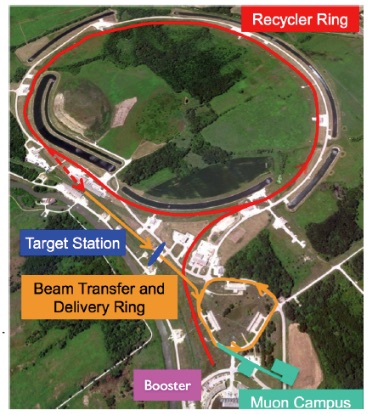
\includegraphics[height=95mm]{MuonCampus.jpg}}
\caption[ Muon Campus Fermi Lab]{ Illustration of the Muon Campus at Fermi Lab  Ref. \cite{MuonCampus}
	}
\label{fig:MuonCampus}
\end{figure}	


	The muon are injected  through the inflector magnet which provides a region free of magnetic fields for the muon to pass through and into the storage ring at MC1. The muons are then centered in the ring using a kicker which is a series of three long plate that are able to produce a pulsed magnetic field. The magnetic field in the ring is produced by super conducting coils surrounded by iron yokes as to maintain uniformity of the magnetic field. Refer to Fig. \ref{fig:SRCrossSection} for a cross section schematic of the ring. As the polarized muons pass through this magnetic field they precess according to the $\omega_a$ frequency as covered in previous sections. The muon then decays into a positron preferentially in the direction of it's spin and is detected by the calorimeters and the tracker stations one the inside of the ring. Shown in Fig. \ref{fig:RingBirdsEye} is a birds eye view representation of the storage ring and the position of the kickers, inflector, tracker stations, and calorimeter stations. The detectors consist of 24 calorimeters and 2 tracker stations that consist of 8 trackers. 
	
\begin{figure}
\centerline{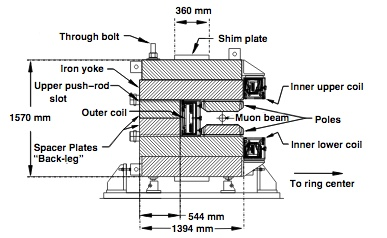
\includegraphics[height=95mm]{RingCrossSection.jpeg}}
\caption[Storage Ring Cross Section]{ Illustration of the cross section of the storage ring  Ref. \cite{TDR}
	}
\label{fig:SRCrossSection}
\end{figure}	
	

\begin{figure}
\centerline{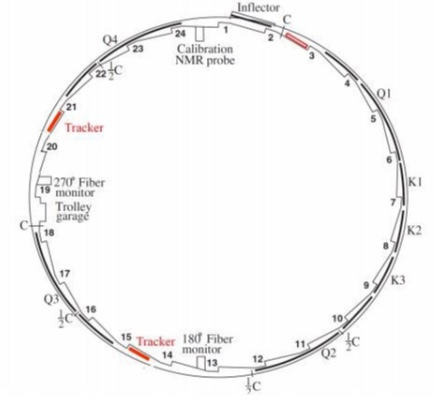
\includegraphics[height=95mm]{RingBirdsEye.jpeg}}
\caption[Birds Eye View of Ring]{ Birds Eye View of the Ring Ref. \cite{TDR}
	}
\label{fig:RingBirdsEye}
\end{figure}	



	Since uncertainties are extremely important in this experiment measurement and evaluation of the uniformity of the magnetic field is necessary. One system used for this are fixed NMR probes at several locations around the ring. A trolley system was developed that can travel throughout the ring and measure the magnetic field. 

\section{Requirements of the E989 Experiment}
	To meet the goal of an experimental precision of 140 ppb, 21 times more data needs to be collected than the E821 experiment. This will result in a 100 ppb statistical uncertainty in the $a_\mu$ measurement. The measurement of $\omega_a$ and $\omega_p$ have a total proposed uncertainty of 70 ppb. The proposed limits for the expected uncertainty of the experiment can be found in Fig. \ref{fig:wauncertainty} and Fig.\ref{fig:wpuncertainty}.

\begin{figure}
\centerline{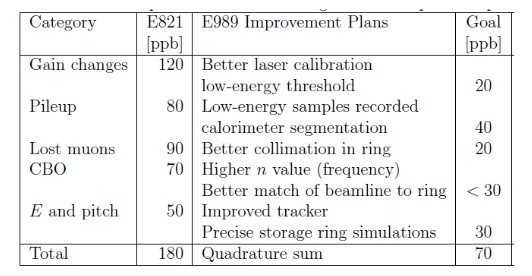
\includegraphics[height=60mm]{wauncertainty.jpeg}}
\caption[Expected improvement of $\omega_a$ measurement in E989]{ Expected Improvement in the systematic uncertainties for $\omega_a$ . Ref \cite{TDR}
	}
\label{fig:wauncertainty}
\end{figure}

\begin{figure}
\centerline{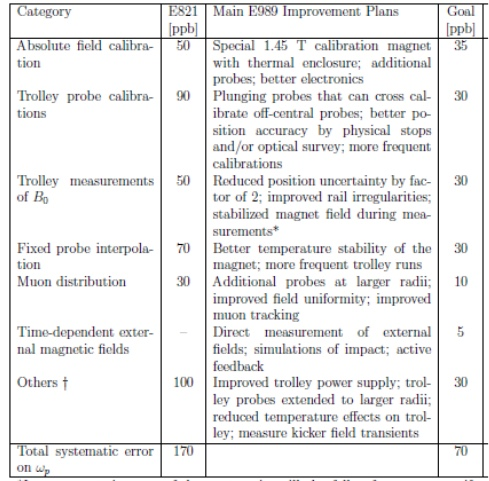
\includegraphics[height=120mm]{wpuncertainty.jpeg}}
\caption[Expected improvement of $\omega_p$ measurement in E989]{ Expected Improvement in the systematic uncertainties for $\omega_p$. Ref. \cite{TDR}
	}
\label{fig:wpuncertainty}
\end{figure}

\section{Current  Status of the Experiment}


\end{document}
